\documentclass[aspectratio=169,10pt]{beamer}

\usetheme{Madrid}
\usecolortheme{default}

\usepackage{amsmath}
\usepackage{amssymb}
\usepackage{booktabs}
\usepackage{graphicx}
\usepackage{pgfplots}

\pgfplotsset{compat=1.18}
\graphicspath{{../output/}}

\definecolor{pgoBlue}{RGB}{37,84,150}
\definecolor{pgoGreen}{RGB}{54,130,91}
\definecolor{pgoOrange}{RGB}{191,104,43}

\setbeamercolor{structure}{fg=pgoBlue}
\setbeamercolor{alerted text}{fg=pgoOrange}
\setbeamertemplate{navigation symbols}{}
\setbeamertemplate{caption}[numbered]

\newcommand{\good}[1]{\textcolor{pgoGreen}{#1}}
\newcommand{\warn}[1]{\textcolor{pgoOrange}{#1}}
\newcommand{\vect}[1]{\operatorname{vec}\!\left(#1\right)}
\newcommand{\norm}[1]{\left\lVert #1\right\rVert}
\newcommand{\eref}{E_{\mathrm{ref}}}

\title[Systematic Poking Calibration]{Systematic Poking Material Calibration}
\subtitle{From Synthetic Neo-Hookean Stresses to Positive-Parameter Gauss--Newton}
\author{libpgo constitutive calibration experiment}
\date{July 2026}

\begin{document}

\begin{frame}
  \titlepage
\end{frame}

\begin{frame}{Question, Goal, and Scope}
  \begin{block}{Question}
    Given deformation gradients and target first Piola stresses
    \[
      \mathcal D=\{(F_c,P_c^{\star})\}_{c=1}^{N},
    \]
    can the paper-style Systematic Poking parameters be fitted robustly using
    analytic parameter derivatives?
  \end{block}

  \vspace{0.4em}
  \begin{columns}[T]
    \begin{column}{0.49\linewidth}
      \textbf{Covered here}
      \begin{itemize}
        \item 17 stretch-curvature parameters
        \item One volumetric coefficient $\lambda$
        \item $P(F)$ residual and analytic Jacobian
        \item Positive-parameter Gauss--Newton
        \item Train/holdout evaluation and linear oracle
      \end{itemize}
    \end{column}
    \begin{column}{0.49\linewidth}
      \textbf{Not covered yet}
      \begin{itemize}
        \item Unknown equilibrium state $u^\star(e)$
        \item Poking contact and force curves
        \item Equilibrium sensitivity
        \item Collapse and inversion extension
      \end{itemize}
    \end{column}
  \end{columns}
\end{frame}

\begin{frame}{Target: Compressible Neo-Hookean Material}
  \small
  Given Young's modulus $E$ and Poisson ratio $\nu$,
  \[
    \mu=\frac{E}{2(1+\nu)},
    \qquad
    \lambda=\frac{E\nu}{(1+\nu)(1-2\nu)}.
  \]

  For principal stretches $s_1,s_2,s_3>0$ and
  $J=s_1s_2s_3$,
  \[
    \psi_{\mathrm{NH}}
    =
    \sum_{i=1}^{3}
    \left[
      \frac{\mu}{2}(s_i^2-1)-\mu\log s_i
    \right]
    +
    \frac{\lambda}{2}(\log J)^2.
  \]

  Therefore, the one-dimensional Valanis--Landel stretch term satisfies
  \[
    f_{\mathrm{NH}}''(s)
    =
    \mu\left(1+\frac{1}{s^2}\right).
  \]

  \begin{block}{Synthetic ground truth}
    $E^\star=2.0\times10^5,\ \nu^\star=0.35$.
    The initial guess uses $E_0=1.2\times10^5,\ \nu_0=0.25$.
  \end{block}
\end{frame}

\begin{frame}{Fitted Model: Paper-Style Systematic Poking}
  \small
  \[
    \psi_{\mathrm{SP}}(s_1,s_2,s_3;e)
    =
    \sum_{i=1}^{3} f(s_i;q)
    +
    \lambda\,\widehat h(J).
  \]

  Stretch curvature uses piecewise-linear hat functions:
  \[
    f''(s;q)=\sum_{k=0}^{K-1}q_k\phi_k(s),
    \qquad q_k=f''(s_k).
  \]
  The spline is integrated subject to
  \[
    f(1)=0,\qquad f'(1)=0.
  \]

  The volumetric spline shape is fixed by log-squared curvature samples:
  \[
    \widehat h''(J_k)
    =
    \frac{1-\log J_k}{J_k^2},
    \qquad
    \widehat h(1)=\widehat h'(1)=0.
  \]

  \[
    e=
    \begin{bmatrix}
      q_0&\cdots&q_{16}&\lambda
    \end{bmatrix}^{T}\in\mathbb R^{18}.
  \]
\end{frame}

\begin{frame}{Positive-Domain Constraint via Log Parameters}
  \small
  Direct optimization over $e$ can produce negative curvature. Instead, use
  \[
    e_i=\eref\exp(\theta_i),
    \qquad \theta_i\in\mathbb R.
  \]

  The complete optimization trajectory then satisfies
  \[
    q_k>0,\qquad \lambda>0.
  \]

  The initial parameters are sampled from the initial Neo-Hookean material:
  \[
    q_{k,0}
    =
    \mu_0\left(1+\frac{1}{s_k^2}\right),
    \qquad
    \lambda_0
    =
    \frac{E_0\nu_0}{(1+\nu_0)(1-2\nu_0)}.
  \]

  \begin{alertblock}{Numerical role}
    The variables $\theta$ are dimensionless. Scaling by $\eref$ gives
    stress-scale physical parameters, removes inequality constraints, and
    prevents line search from leaving the positive parameter domain.
  \end{alertblock}
\end{frame}

\begin{frame}{Experiment Design: Deformation Coverage}
  \small
  \begin{table}
    \centering
    \begin{tabular}{lccp{0.39\linewidth}}
      \toprule
      family & train & holdout & role \\
      \midrule
      uniaxial & 8 & 7 & tension/compression and volume coupling \\
      biaxial & 6 & 6 & repeated principal stretches \\
      volumetric & 6 & 6 & primarily identify $\lambda$ \\
      isochoric & 6 & 6 & separate stretch and volume responses \\
      simple shear & 6 & 6 & non-diagonal $F$ \\
      rotated distinct & 12 & 18 & general $F$ and rotational invariance \\
      knot-aligned uniaxial & 16 & 0 & excite every curvature basis function \\
      \midrule
      total & 60 & 49 & disjoint random samples \\
      \bottomrule
    \end{tabular}
  \end{table}

  Stretch knots are 17 log-uniform points on $[0.5,2]$.
  Volume knots are 17 log-uniform points on $[e^{-1},e]$.
\end{frame}

\begin{frame}{Extracting $P(F)$ from Affine FEM Energy}
  \small
  Prescribe affine displacement on a unit cube:
  \[
    u_a(F)=(F-I)X_a.
  \]

  Define
  \[
    B=\frac{\partial u}{\partial\vect{F}},
    \qquad
    g(u,e)=\frac{\partial E_h(u,e)}{\partial u}.
  \]

  Discrete virtual work gives
  \[
    \delta E_h
    =
    g^T\delta u
    =
    g^TB\,\delta\vect{F}
    =
    V\,\vect{P}^{\,T}\delta\vect{F},
  \]
  and therefore
  \[
    \boxed{
      \vect{P(F,e)}
      =
      \frac{1}{V}B^Tg(u(F),e)
    }.
  \]

  Here $V=1$. Since $F$ is prescribed, this is direct constitutive
  evaluation and \alert{does not require a static solve}.
\end{frame}

\begin{frame}{Loss: Normalized Stress Residual}
  \small
  For deformation case $c$,
  \[
    r_c(\theta)
    =
    \frac{
      \vect{P_{\mathrm{SP}}(F_c;e(\theta))
      -
      P_{\mathrm{NH}}(F_c)}
    }{\eref}
    \in\mathbb R^9.
  \]

  Stack all training cases:
  \[
    r(\theta)
    =
    \begin{bmatrix}
      r_1(\theta)\\
      \vdots\\
      r_N(\theta)
    \end{bmatrix},
    \qquad
    \boxed{
      \Phi(\theta)=\frac12\norm{r(\theta)}_2^2
    }.
  \]

  \begin{block}{Why divide by $\eref$?}
    The residual, Jacobian, and objective become dimensionless, preventing the
    $\mathcal O(10^5)$ material scale from degrading numerical conditioning.
  \end{block}
\end{frame}

\begin{frame}{Analytic Parameter Jacobian}
  \small
  FEM provides the mixed derivative
  \[
    E_{ue}
    =
    \frac{\partial^2E_h}{\partial u\,\partial e}.
  \]

  At fixed $F$,
  \[
    \frac{\partial\vect{P}}{\partial e}
    =
    \frac1V B^TE_{ue}.
  \]

  Using
  \[
    \frac{\partial e_i}{\partial\theta_j}
    =
    e_i\delta_{ij},
  \]
  gives the per-case Jacobian
  \[
    \boxed{
      \frac{\partial r_c}{\partial\theta}
      =
      \frac1{V\eref}
      B^TE_{ue}\operatorname{diag}(e)
    }.
  \]

  Central finite-difference verification:
  \[
    \frac{\norm{J-J_{\mathrm{FD}}}_F}
         {\norm{J_{\mathrm{FD}}}_F}
    =4.8\times10^{-10}.
  \]
\end{frame}

\begin{frame}{Damped Gauss--Newton with Line Search}
  \small
  At each iteration,
  \[
    g_\theta=J^Tr,
    \qquad
    H_{\mathrm{GN}}=J^TJ,
  \]
  and the step solves
  \[
    \boxed{
      \left[
        J^TJ+\gamma\,\operatorname{diag}(J^TJ)
      \right]\Delta\theta
      =
      -J^Tr
    }.
  \]

  \begin{enumerate}
    \item Restrict $\norm{\Delta\theta}_\infty\leq1$ to avoid exponential jumps.
    \item Backtrack over $\alpha\in\{1,\frac12,\frac14,\ldots\}$.
    \item Accept a step when $\Phi(\theta+\alpha\Delta\theta)<\Phi(\theta)$.
    \item On success, set $\gamma\leftarrow\gamma/3$; on failure,
      set $\gamma\leftarrow10\gamma$.
    \item Stop on gradient tolerance, step tolerance, or failure to decrease.
  \end{enumerate}
\end{frame}

\begin{frame}{Key Diagnosis: Why Was the Initial Design Rank Deficient?}
  \small
  \begin{columns}[T]
    \begin{column}{0.48\linewidth}
      \begin{alertblock}{Initial setup}
        Every observed stretch lay strictly inside $(0.5,2)$. The two endpoint
        hat functions never entered an integration interval, so
        \[
          \operatorname{rank}(A)=16<18.
        \]
        The outer parameters were unidentifiable, and the unconstrained oracle
        contained zero and negative entries.
      \end{alertblock}
    \end{column}
    \begin{column}{0.48\linewidth}
      \begin{block}{Corrected setup}
        Add one training state at every non-rest knot:
        \[
          F_k=\operatorname{diag}(s_k,1,1).
        \]
        The corrected design has
        \[
          \operatorname{rank}(A)=18,
          \qquad
          \kappa(A)=800.3.
        \]
      \end{block}
    \end{column}
  \end{columns}

  \vspace{0.7em}
  \centering
  \textbf{An optimizer cannot recover material directions that the data never excite.}
\end{frame}

\begin{frame}{Independent Check: Linear Oracle in Physical Parameters}
  \small
  The integrated-curvature spline is linear in its curvature samples, and the
  volume term is linear in $\lambda$. Thus, at fixed $F$,
  \[
    \vect{P_{\mathrm{SP}}(F;e)}=A(F)e.
  \]

  Across all training cases, construct
  \[
    A\bar e\approx b,
    \qquad
    \bar e=\frac{e}{\eref},
    \qquad
    b=\frac{\vect{P^\star}}{\eref}.
  \]

  The unconstrained linear optimum is
  \[
    \bar e_{\mathrm{oracle}}
    =
    \arg\min_{\bar e}\norm{A\bar e-b}_2^2.
  \]

  \begin{block}{Current experiment}
    All 18 oracle parameters are positive. The relative difference between
    Gauss--Newton and the oracle is
    \[
      \frac{\norm{e_{\mathrm{GN}}-e_{\mathrm{oracle}}}_2}
           {\norm{e_{\mathrm{oracle}}}_2}
      =5.7\times10^{-14}.
    \]
  \end{block}
\end{frame}

\begin{frame}{Optimization Convergence}
  \begin{columns}[T]
    \begin{column}{0.66\linewidth}
      \centering
      \begin{tikzpicture}
        \begin{semilogyaxis}[
          width=\linewidth,
          height=0.65\textheight,
          xlabel={iteration},
          ylabel={objective $\Phi$},
          grid=both,
          ymin=1e-5,
          ymax=2e1,
          xtick={0,1,2,3,4,5},
          mark size=2.5pt,
        ]
          \addplot[
            color=pgoBlue,
            very thick,
            mark=*,
          ] coordinates {
            (0,9.09432296)
            (1,1.18888281)
            (2,3.09831168e-2)
            (3,3.51171478e-5)
            (4,2.53631108e-5)
            (5,2.53631096e-5)
          };
        \end{semilogyaxis}
      \end{tikzpicture}
    \end{column}
    \begin{column}{0.31\linewidth}
      \small
      \begin{itemize}
        \item Six iterations to gradient tolerance
        \item The first three iterations make the dominant reduction
        \item Final objective:
          \[
            \Phi=2.54\times10^{-5}
          \]
        \item The remaining floor is dominated by finite-knot spline
          approximation
      \end{itemize}
    \end{column}
  \end{columns}
\end{frame}

\begin{frame}{Fit Diagnostics: Parameters, Convergence, and Holdout}
  \centering
  \includegraphics[width=0.98\linewidth]{fit_diagnostics.png}

  \vspace{-0.4em}
  \scriptsize
  Left: fitted $f''$ tracks analytic Neo-Hookean curvature.
  Center: rapid objective convergence.
  Right: holdout stress components lie close to $y=x$.
\end{frame}

\begin{frame}{Quantitative Results}
  \small
  \begin{table}
    \centering
    \begin{tabular}{lrrr}
      \toprule
      split & initial RMSE & fitted RMSE & reduction \\
      \midrule
      training & $1.8353\times10^{-1}$ & $3.0649\times10^{-4}$ & $598.8\times$ \\
      holdout & $1.4709\times10^{-1}$ & $2.4385\times10^{-4}$ & $603.2\times$ \\
      \bottomrule
    \end{tabular}
  \end{table}

  \vspace{0.7em}
  \begin{columns}[T]
    \begin{column}{0.48\linewidth}
      \begin{block}{Optimization result}
        \begin{itemize}
          \item All 18 parameters are identifiable
          \item Every fitted parameter is positive
          \item Holdout data are excluded from optimization
          \item Training and holdout errors have the same scale
        \end{itemize}
      \end{block}
    \end{column}
    \begin{column}{0.48\linewidth}
      \begin{block}{Implementation checks}
        \begin{itemize}
          \item FEM/linear-model difference: $2.2\times10^{-16}$
          \item Jacobian FD relative difference: $4.8\times10^{-10}$
          \item Python: 64 tests passed
          \item Related C++: 28 tests passed
        \end{itemize}
      \end{block}
    \end{column}
  \end{columns}
\end{frame}

\begin{frame}{Knot-Resolution Sweep}
  \small
  \begin{table}
    \centering
    \begin{tabular}{rrrrr}
      \toprule
      knots & parameters & rank & $\kappa(A)$ & holdout RMSE \\
      \midrule
      5  & 6  & 6  & $7.01\times10^1$ & $4.67\times10^{-3}$ \\
      9  & 10 & 10 & $2.11\times10^2$ & $1.00\times10^{-3}$ \\
      17 & 18 & 18 & $8.00\times10^2$ & $2.44\times10^{-4}$ \\
      33 & 34 & 34 & $3.80\times10^3$ & $7.54\times10^{-5}$ \\
      \bottomrule
    \end{tabular}
  \end{table}

  \vspace{0.8em}
  \begin{block}{Interpretation}
    Increasing knot count decreases representation error while increasing the
    design condition number. The noiseless synthetic problem remains stable;
    real noisy data will eventually require curvature smoothness
    regularization, dimensionality reduction, or cross-validated knot count.
  \end{block}
\end{frame}

\begin{frame}{Why This Experiment Does Not Need a Static Solve}
  \small
  Here $F$ is prescribed, so the forward map is
  \[
    (F,e)\longmapsto P(F,e).
  \]
  The displacement $u(F)$ is known; the energy gradient is evaluated directly.

  In a real poking fit, displacement is defined implicitly by equilibrium:
  \[
    R(u^\star,e)
    =
    \frac{\partial\Pi(u^\star,e)}{\partial u}
    =0.
  \]
  The forward chain becomes
  \[
    e\longmapsto u^\star(e)
    \longmapsto F(u^\star)
    \longmapsto P,\;f_{\mathrm{contact}}
    \longmapsto L,
  \]
  and requires
  \[
    \boxed{
      \frac{du^\star}{de}
      =
      -
      \left(\frac{\partial R}{\partial u}\right)^{-1}
      \frac{\partial R}{\partial e}
    }.
  \]
\end{frame}

\begin{frame}{Conclusions and Next Step}
  \begin{block}{Supported by this experiment}
    \begin{itemize}
      \item Systematic Poking parameters, FEM stress, and mixed derivatives
        form a complete optimization chain.
      \item Log parameterization preserves positive curvature and positive
        $\lambda$ without constrained optimization.
      \item Knot-domain coverage is necessary for parameter identifiability.
      \item Analytic Jacobians, the linear oracle, and holdout data provide
        independent and mutually consistent validation.
    \end{itemize}
  \end{block}

  \vspace{0.5em}
  \begin{alertblock}{Next step}
    First add stress noise and curvature smoothness regularization. Then replace
    direct stress residuals with poking force--displacement observations and
    optimize through equilibrium and contact sensitivity.
  \end{alertblock}

  \vfill
  \scriptsize
  Reference: Chen, Zhao, and Barbi\v{c},
  \emph{Capturing Animation-Ready Isotropic Materials Using Systematic Poking},
  ACM TOG 42(6), 2023.
\end{frame}

\end{document}
